\section{image}
The camera plus the lens converts the information in the three-dimensional world into a photo of pixels, which is then stored in the computer as a source of data for subsequent processing. In mathematics, images can be described by a matrix; in a computer, they occupy a contiguous disk or memory space, which can be represented by a two-dimensional array. In this way, the program does not have to distinguish whether they are dealing with a numerical matrix or a meaningful image.

In this section, we will introduce some basic operations of computer image processing. In particular, through the processing of image data in OpenCV, the common steps of processing images in a computer are understood to lay the foundation for subsequent chapters. Let's start with the simplest image, the grayscale image. In a grayscale image, each pixel position $(x, y)$ corresponds to a gray value of $I$, so an image with a width of $w$ and a height of $h$ can be mathematically recorded. As a function:

\[
{I} (x,y): \mathbb{R}^2 \mapsto \mathbb{R}.
\]

Where $(x,y)$ is the coordinates of the pixel. However, the computer does not express real space, so we need to quantify the subscript and image readings within a certain range. For example $x, y$ is usually an integer starting at 0. In a common grayscale image, an integer of 0\textasciitilde255 (ie, an unsigned char, 1 byte) is used to represent the grayscale reading of the image. Then, a grayscale image with a width of 640 pixels and a height of 480 pixels can be expressed as:

\begin{lstlisting}[language=C++, caption=two-dimensional array representation image]
Unsigned char image[480][640];
\end{lstlisting}

Why is the 2D array here 480$\times$640? Because in the program, the image is stored as a two-dimensional array. Its first subscript is the row of the exponent group, and the second subscript is the column. In an image, the number of rows in an array corresponds to the height of the image, and the number of columns corresponds to the width of the image.

Let's examine the content of this image. The image is naturally composed of pixels. When accessing a pixel, you need to indicate the coordinates it is in, as shown by \autoref{fig:imagesInComputer}~. The left side of the figure shows how the traditional pixel coordinate system is defined. The origin of the pixel coordinate system is in the upper left corner of the image, $X$ is axially right, and $Y$ is axially down (that is, the $u, v$ coordinates mentioned earlier). If it still has a third axis, the $Z$ axis, then according to the right-hand rule, the $Z$ axis should be forward. This definition is consistent with the camera coordinate system. The width or number of columns we usually say corresponds to the $X$ axis; the number of rows or height of the image corresponds to its $Y$ axis.

\begin{figure}[!t]
	\centering
	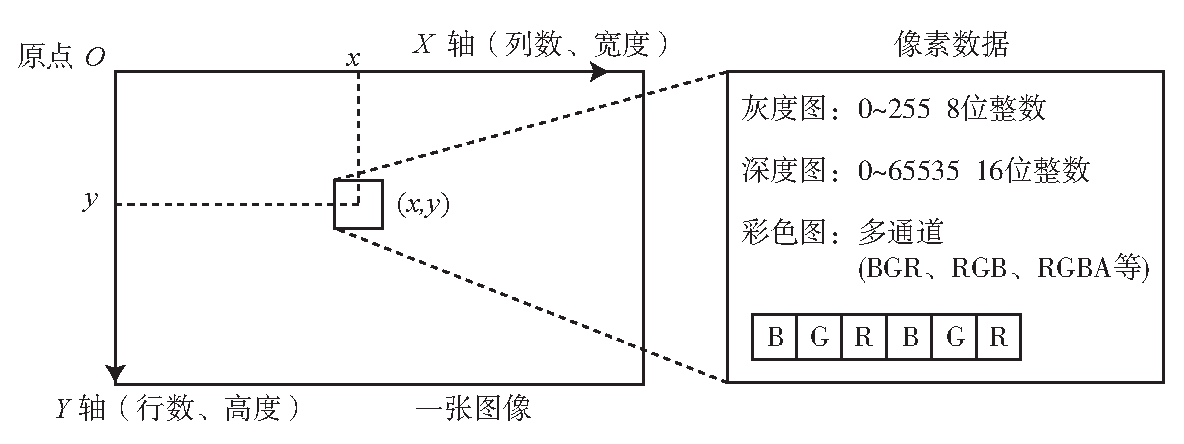
\includegraphics[width=0.84\textwidth]{chapter05/resources/cameraModel/image.pdf}
	\caption{Image coordinate diagram. }
	\label{fig:imagesInComputer}
\end{figure}

According to this definition, if we discuss a pixel at $x,y$, then its access in the program should be:

\begin{lstlisting}[language=C++, caption=Access Image Pixels]
Unsigned char pixel = image[y][x];
\end{lstlisting}

It corresponds to a reading of the gray value $I(x,y)$. Please note the order of $x$ and $y$ here. Although we are tired of discussing the problem of the coordinate system, errors like this subscript order will still be one of the mistakes that novices often encounter during the debugging process, and have some concealment errors. If you accidentally change the coordinates of $x,y$ while writing the program, the compiler can't provide any information, and all you can see is an out-of-bounds error in the running of the program.

The gray level of a pixel can be recorded with an 8-bit integer, which is a value of 0\textasciitilde255. When we have more information to record, one byte is probably not enough. For example, in the depth map of the RGB-D camera, the distance between each pixel and the camera is recorded. This distance is usually in millimeters, while the range of RGB-D cameras is usually around a dozen meters, more than 255. At this time, people will use a 16-bit integer (unsigned short in C++) to record the depth map information, that is, the value at 0\textasciitilde65535. When converted to meters, the maximum can be 65 meters, enough for RGB-D cameras.

The representation of a color image requires the concept of a channel.
In the computer, we use a combination of three colors of red, green and blue to express any color.Therefore, for each pixel, three values of R, G, and B are recorded, and each value is called a channel. For example, the most common color image has three channels, each represented by an 8-bit integer. Under this rule, one pixel occupies a 24-bit space.

The number and order of channels are freely definable. In OpenCV color images, the default order of channels is B, G, R. That is, when we get a 24-bit pixel, the first 8 bits represent the blue value, the middle 8 bits are green, and the last 8 bits are red. Similarly, a color map can be represented by the order of R, G, and B. If you want to express the transparency of the image, use the four channels R, G, B, and A.
